% Gemini theme
% https://github.com/anishathalye/gemini
%
% This project includes software licensed under the MIT License.
% Copyright (c) Anish Athalye

\documentclass[final]{beamer}

% ====================
% Packages
% ====================

\usepackage[T1]{fontenc}
\usepackage{lmodern}
\usepackage{caption}
% \usepackage[size=custom,width=118.9,height=84.1,scale=1.0]{beamerposter}
\usepackage[size=custom,width=84.1,height=118.9,scale=1.0]{beamerposter}


% \makeatletter
% \def\input@path{{colorthemes/}}
% \makeatother

\usetheme{gemini}
\usecolortheme{itu}
\usepackage{graphicx}
\usepackage{booktabs}
\usepackage{tikz}
\usepackage{pgfplots}
\pgfplotsset{compat=1.14}
\usepackage{anyfontsize}

\makeatletter
\renewcommand{\@cite}[2]{\textsuperscript{[#1\if@tempswa , #2\fi]}}
\makeatother

% ====================
% Lengths
% ====================

% If you have N columns, choose \sepwidth and \colwidth such that
% (N+1)*\sepwidth + N*\colwidth = \paperwidth
\newlength{\sepwidth}
\newlength{\colwidth}
\setlength{\sepwidth}{0.033\paperwidth}
\setlength{\colwidth}{0.45\paperwidth}

\newcommand{\separatorcolumn}{\begin{column}{\sepwidth}\end{column}}

% ====================
% Title
% ====================

\title{
% \hspace*{\sepwidth}\RaggedRight
NanoTabPFN Pretraining Speedrun
% \newline\hspace*{\sepwidth}
}

\author{Salih \underline{Bora} Öztürk \inst{1} \and Alexander Pfefferle \inst{2,1} \and Frank Hutter \inst{3,2,1}}

\institute[shortinst]{\inst{1} University of Freiburg \samelineand \inst{2} ELLIS Institute Tübingen \samelineand \inst{3} Prior Labs}

% ====================
% Footer (optional)
% ====================

\footercontent{
  \parbox[c][8cm][c]{\textwidth}{
    \hspace{2em}
    
\includegraphics[height=4.1cm]{img/logo_ellis_horizontal.png}
    \hfill
    
\includegraphics[height=4.8cm]{img/logo_automl.png}
    \hfill
    
\includegraphics[height=3.9cm]{img/logo_prior_horizontal.png}
    \hspace{3em}
  }
}
% (can be left out to remove footer)

% ====================
% Logo (optional)
% ====================

% use this to include logos on the left and/or right side of the header:
\logoright{
\includegraphics[height=9cm]{img/logo_ufr_circle_black.png}}
% \logoleft{\includegraphics[height=7cm]{logo2.pdf}}

% ====================
% Body
% ====================

\begin{document}

\begin{frame}[t]

\begin{columns}[t]
\separatorcolumn
\begin{column}{0.934\paperwidth}
  \begin{block}{Architectural changes}
    \centering
    
\includegraphics[width=0.84\linewidth]{img/base.png}

    \smallskip
    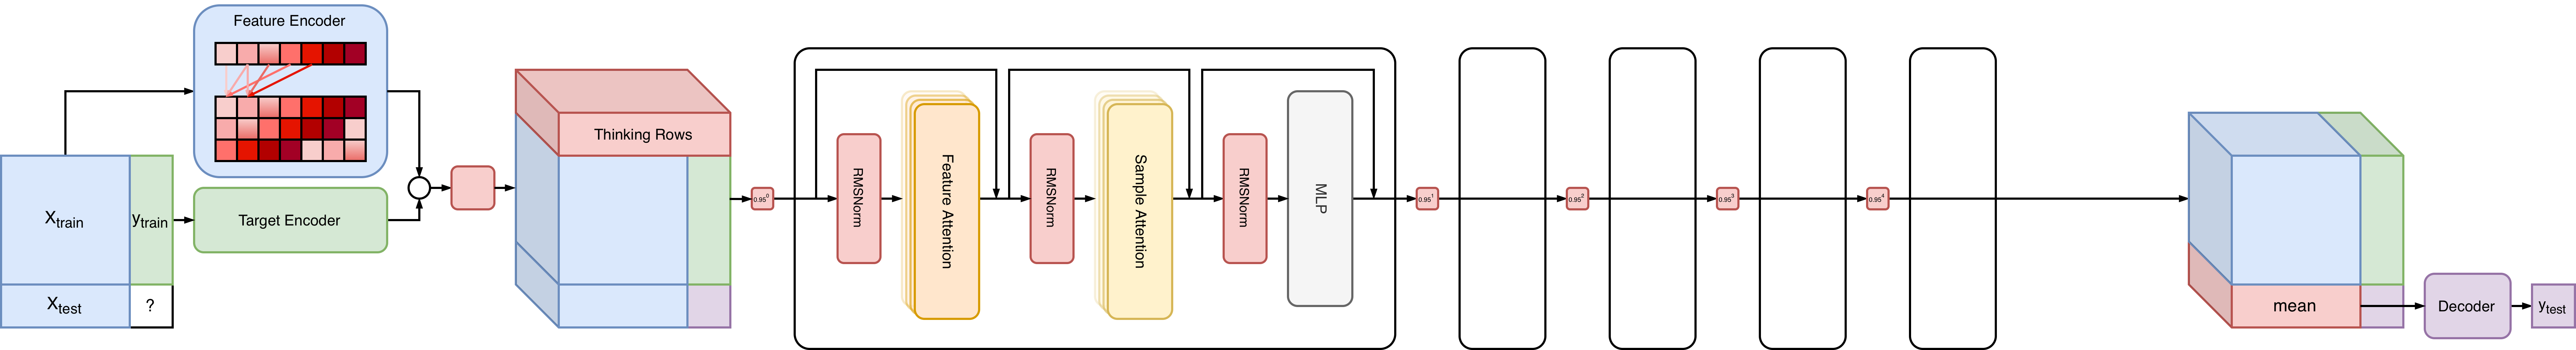
\includegraphics[width=0.84\linewidth]{img/modded.png}

    \smallskip
    {\small Baseline (top) vs.\ current record (bottom, changes in red): grouped feature encoding, 24 thinking rows, pre-attention RMSNorms, residual decay $0.95^i$, 5 blocks, mean feature pooling.}
  \end{block}
\end{column}
\separatorcolumn
\end{columns}

\begin{columns}[t]
\separatorcolumn

\begin{column}{0.46\paperwidth}

  \begin{alertblock}{TL;DR}

    \textbf{modded-nanoTabPFN}: This repository hosts the nanoTabPFN speedrun, in which we search for the fastest way to train a tabular foundation model that beats Random Forest on TabArena datasets.

  \end{alertblock}

  \begin{block}{Speedrun overview}

    \heading{Motivation}

      \begin{itemize}
        \item TabPFN have shown that pretraining on synthetic datasets can lead to strong performance... \cite{hollmann2023tabpfn} \cite{hollmann2025tabpfnv2}
        \item However, training these models takes long, and no one has time to wait...
      \end{itemize}

    \heading{Background}

    \begin{itemize}
        \item GPT2  →  nanoGPT  →  modded-nanoGPT (45 mins to 1.54 mins)
        \item TabPFNv2 → nanoTabPFN → modded-nanoTabPFN (75 mins to 0.92 mins)
      \end{itemize}

    \heading{Goal}

      \begin{itemize}
        \item Pretrain a neural network to beat Random Forest (\textasciitilde 0.8068 validation average ROC AUC) on subsampled TabArena datasets using 1 NVIDIA L40S.
      \end{itemize}

    \heading{This repo now contains a training algorithm which attains the target performance in:}

      \begin{itemize}
        \item \textbf{0.92 minutes} on 1xL40S (baseline needed 74.32)
        \item \textbf{3648 synthetic datasets} (baseline needed 80576)
      \end{itemize}

    \heading{Timing protocol}

    \begin{itemize}
      \item Counting only training wall-clock time (forward/backward/optimizer steps over synthetic batches).
      \item Evaluation runtime is excluded.
      \begin{itemize}
        \item the training timer is stopped while running validation.
      \end{itemize}
      \item Prior generation time is excluded.
      \begin{itemize}
        \item using a pre-generated prior dump is allowed.
      \end{itemize}
    \end{itemize}

    \heading{Evaluation is on all 38 TabArena classification datasets:}

    \begin{itemize}
      \item if >100 features, randomly select 100
      \item if >1000 rows, randomly select 1000 (stratified by class labels)
      \item 5-fold StratifiedKFold with shuffling, class labels are encoded with integers per fold
      \item average binary or one-vs-rest ROC AUC over all datasets
    \end{itemize}

    \heading{New records must:}

    \begin{enumerate}
      \item Not modify the evaluation pipeline.
      \item Not load any pretrained weights.
      \item Run faster than prior record when baselined on the same hardware.
    \end{enumerate}

    Other than that, anything and everything is fair game, including changes to the synthetic prior generation!

    \vspace{0.7em}

    \heading{This improvement in training speed has been brought about by the following techniques:}

    \begin{minipage}[t]{0.49\linewidth}
      \begin{itemize}
        \item Muon optimizer \cite{jordan2024muon}
        \item Batched Muon zeropower for grouped QKV
        \item SDPA rewrite with explicit QKV
        \item Pre-norm transformer blocks \cite{geiping2023cramming}
        \item Compiled encoder layer forward
        \item bfloat16 autocast in training and inference
        \item float32 matmul precision high
        \item Learning rate $10^{-4} \rightarrow 10^{-3}$
        \item Embeddings $192 \rightarrow 256$, heads $6 \rightarrow 4$
        \item Exponential residual stream decay
      \end{itemize}
    \end{minipage}\hfill
    \begin{minipage}[t]{0.49\linewidth}
      \begin{itemize}
        \item Lower precision RMSNorm \cite{zhang2019rmsnorm}
        \item 24 learnable Thinking Rows \cite{grinsztajn2026tabpfn25advancingstateart}
        \item LAWA of 10 checkpoints \cite{kaddour2022lawa, sanyal2024early}
        \item Schedule-Free AdamW WD 0.01 \cite{defazio2024schedulefree}
        \item Repeated feature grouping (group size 5) \cite{qu2026tabiclv2}
        \item Autoresearch-driven HPO \cite{karpathy2026autoresearch}
        \begin{itemize}
          \item Layers $6 \rightarrow 5$
          \item Batch size $1 \rightarrow 2$, dump step size $64 \rightarrow 32$
          \item Muon WD 0.1
          \item Muon momentum $0.95 \rightarrow 0.96$
          \item Gradient clip $1.0 \rightarrow 2.0$
          \item Mean test feature pooling into decoder
        \end{itemize}
      \end{itemize}
    \end{minipage}

  \end{block}

\end{column}

\separatorcolumn

\begin{column}{0.44\paperwidth}

  \begin{block}{Record history}

    \begin{figure}
      \centering
      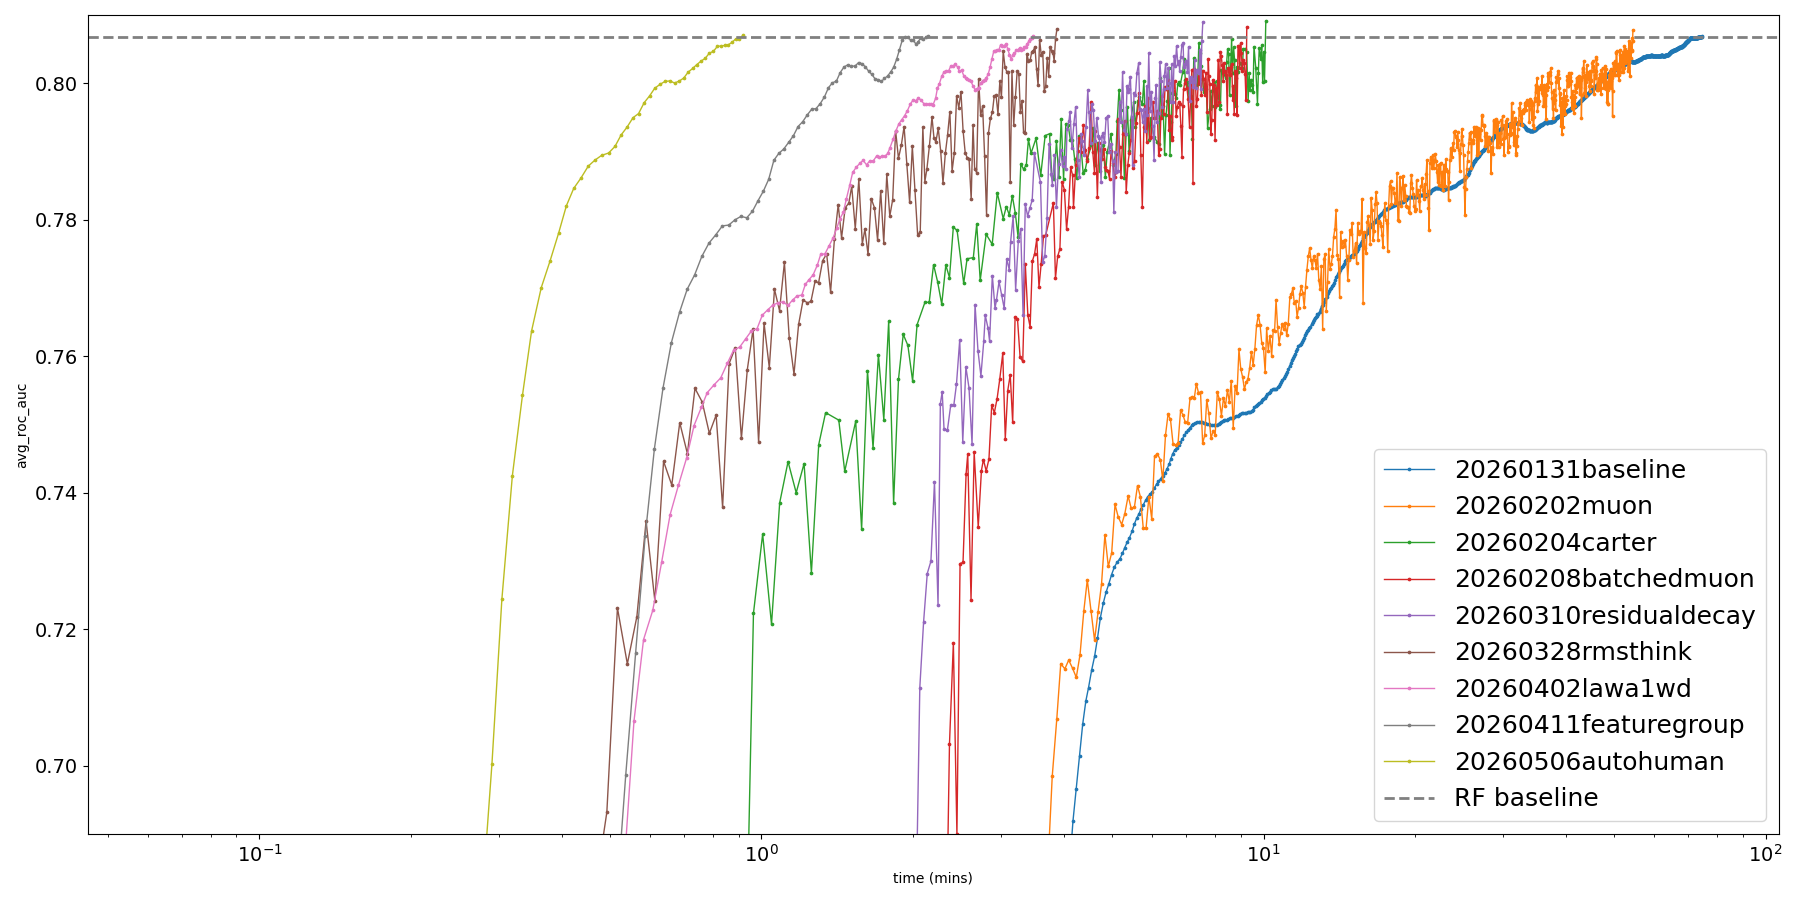
\includegraphics[width=0.95\linewidth]{img/260529-185956-records-plot-x-time-y-val.png}
      \caption*{The baseline lacked modern training tricks, our trick cocktail is \textasciitilde$80\times$ faster.}
      \label{fig:record-history-time}
    \end{figure}

    \begin{center}
      {\normalsize
      \setlength{\tabcolsep}{12pt}
      \begin{tabular}{@{}l p{0.59\linewidth} p{0.18\linewidth}@{}}
        \toprule
        Record time & Description & Contributors \\
        \midrule
        74.32 mins & Baseline & \\
        54.41 mins & Muon optimizer & @borawhocodess \\
        10.10 mins & SDPA, bf16, higher LR, wider embeddings, fewer heads & @carterprince \\
        9.26 mins & Batched Muon, compiled forward & @carterprince \\
        7.57 mins & Exponential decay of residual stream & @borawhocodess \\
        3.88 mins & RMSNorm, Thinking Rows & @borawhocodess \\
        3.48 mins & LAWA, Schedule-Free AdamW WD & @borawhocodess \\
        2.15 mins & Repeated feature grouping & @borawhocodess \\
        0.92 mins & Autoresearch HPO, Muon WD, mean feature pooling & @borawhocodess \\
        \bottomrule
      \end{tabular}
      }
    \end{center}

  \end{block}

  \begin{exampleblock}{Join the race!}

    \begin{figure}
      \centering
      
\includegraphics[width=0.33\linewidth]{img/qr.png}
      \caption*{Scan to join the speedrun on GitHub\\{\footnotesize github.com/borawhocodess/modded-nanotabpfn}}
    \end{figure}

  \end{exampleblock}

  \begin{block}{References}

    \nocite{*}
    \tiny{\bibliographystyle{unsrt}\bibliography{poster}}

  \end{block}

\end{column}

\separatorcolumn
\end{columns}
\end{frame}

\end{document}
